\documentclass[main.tex]{subfiles}


\begin{document}


\section{Results}

\subsection{Workflow of SEARCH-MaP and SEISMIC-RNA}

% In Figure 1, the RNA sequence is CAAUGUGCCAAAGGUCAU (18 nt).
% This sequence could fold into the structures
% ..(((..((...)).))) [P--R base pairs formed] and
% ((...))((...)).... [P--R base pairs unformed].
% Since its purpose is only to illustrate a toy example, this sequence is never specified in the paper.

\begin{figure}[H]
	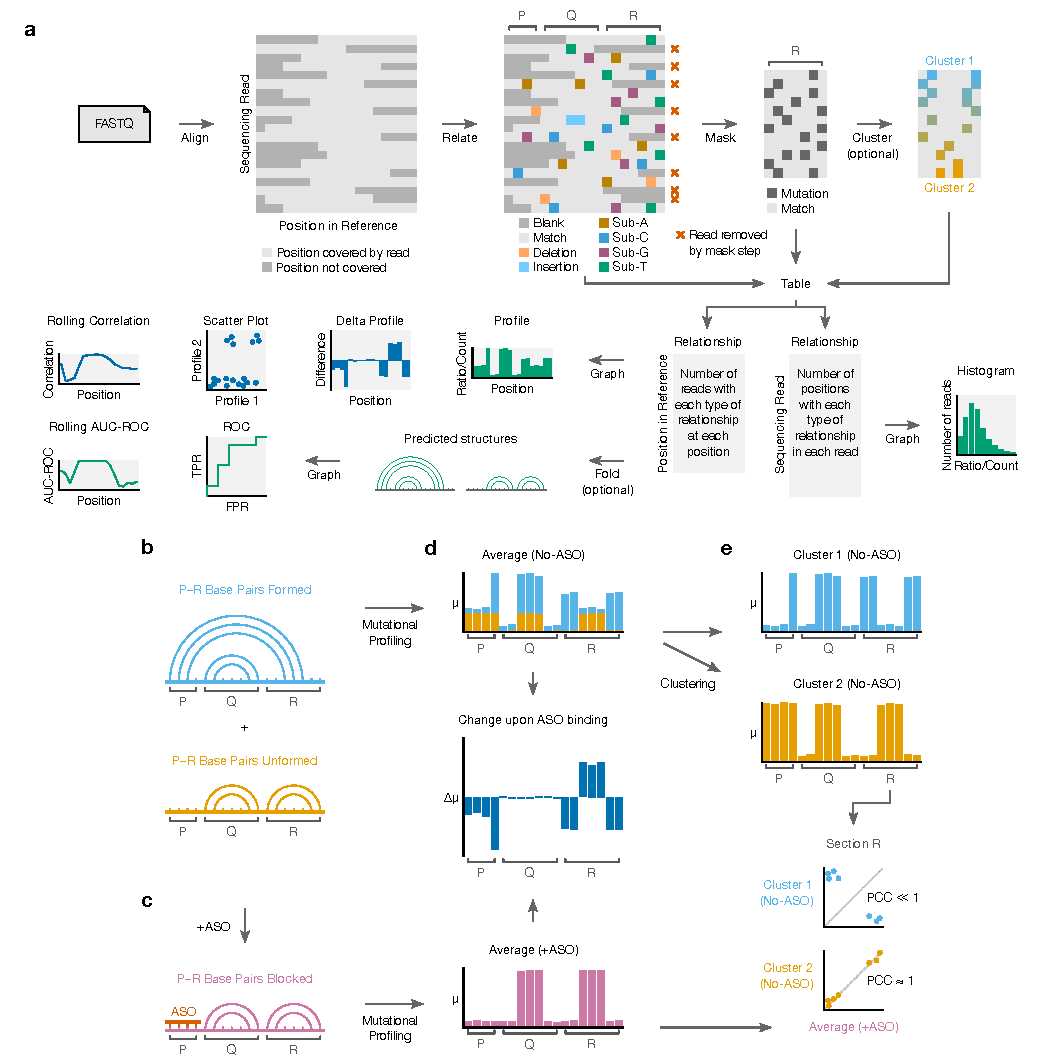
\includegraphics[width=\textwidth]{../MainFigures/wf/wf.pdf}
	\caption{\textbf{The workflow of SEARCH-MaP and SEISMIC-RNA.} (Continued on next page.)}
	\label{strat}
\end{figure}
\addtocounter{figure}{-1}
\begin{figure}[H]
	\caption[]{(Continued from previous page.) \textbf{(a)}~This toy RNA is partitioned into three sections (P, Q, and R) and folds into an ensemble of two structures: one in which base pairs between P and R form and one in which they do not. \textbf{(b)}~Hybridizing an ASO to P blocks it from base-pairing with R. \textbf{(c)}~A SEARCH-MaP experiment entails separate chemical probing and mutational profiling (MaP) with (+ASO) and without (no-ASO) the ASO, followed by sequencing to generate FASTQ files. The RNA molecules and FASTQ files use the same color scheme as in (a) and are illustrated/colored in proportion to their abundances in the ensemble. \textbf{(d)}~Mutational profiles with (+ASO) and without (no-ASO) the ASO, computed as ensemble averages with SEISMIC-RNA. The \textit{x}-axis is the position in the RNA sequence; the \textit{y}-axis is the fraction of mutated bases ($\mu$) at the position. Each bar in the no-ASO profile is drawn in two colors merely to illustrate how many mutations at each position come from each structure; in a real experiment, this information would not exist before clustering. The change upon ASO binding indicates the difference in the fraction of mutated bases ($\Delta \mu$) between the +ASO and no-ASO conditions. \textbf{(e)}~Mutational profiles of two clusters (top) obtained by clustering the no-ASO ensemble in (d) using SEISMIC-RNA, and scatter plots comparing the mutational profiles (bottom) between the +ASO ensemble average (\textit{x}-axis) and each cluster (\textit{y}-axis); each point represents one base in section R. The expected Pearson correlation coefficient (PCC) is shown beside each scatter plot. \textbf{(f)}~The workflow of SEISMIC-RNA. First, sequencing reads (in FASTQ files) are aligned to reference sequence(s). For every read, the relationship to each base in the reference sequence (i.e. match, substitution, deletion, insertion) is determined. In the next step, relationships are called as mutated, matched, or uninformative; and positions and reads failing to meet certain criteria are masked out. Optionally, masked reads can be clustered to reveal alternative structures. The types of relationships at each position and in each read are then counted and tabulated. SEISMIC-RNA can use these tables to predict RNA secondary structures or draw a variety of graphs including mutational profiles, scatter plots, and receiver operating characteristic (ROC) curves.}

\end{figure}

We illustrate SEARCH-MaP with an RNA comprising three sections (P, Q, and R) that folds into an ensemble of two structures: one in which base pairs between P and R form and one in which they do not (Figure~\ref{strat}a).
Searching for base pairs involving section P begins by blocking P with an antisense oligonucleotide (ASO), which ablates the base pairs between P and R (Figure~\ref{strat}b).
The RNA is chemically probed separately with (+ASO) and without (no-ASO) the ASO, followed by mutational profiling (MaP) and sequencing, e.g. using DMS-MaPseq~\cite{Zubradt2016} (Figure~\ref{strat}c).

SEISMIC-RNA can detect base pairs by comparing the +ASO and no-ASO mutational profiles.
Theoretically, each structure has its own mutational profile~\cite{Sherpa2015}, but the mutational profile of a single structure is not directly observable because all structures are physically mixed during the experiment (Figure~\ref{strat}c, top).
Instead, the directly observable mutational profile is of the ``ensemble average" -- the average of the structures' (unobserved) mutational profiles, weighted by the their (unobserved) proportions (Figure~\ref{strat}d, top).
Because the mutational profile of section R changes when it base-pairs with P, the ensemble averages of R differ between the +ASO and no-ASO conditions (Figure~\ref{strat}d, middle).
However, the ASO has little effect on section Q because this section does not base-pair with P (Figure~\ref{strat}d, middle).
Therefore, one can deduce that P interacts with R -- but not with Q -- because hybridizing an ASO to P alters the mutational profile of R but not of Q.

Going one step further, one can resolve the mutational profile where P and R base-pair, even without knowing the exact base pairs.
This step uses SEISMIC-RNA to cluster the no-ASO ensemble into two mutational profiles over section R -- each corresponding to one structure -- and comparing them to the +ASO ensemble average (Figure~\ref{strat}e).
Because the ASO blocks the P--R base pairs, the +ASO mutational profile will correlate better with that of the structure where P and R do not base-pair; in this case, cluster 2 correlates better.
Therefore, the mutational profile of cluster 1 corresponds to the structure where P and R base-pair.

\subsection{SEARCH-MaP finds base pairs in ribosomal RNA}

We first validated SEARCH-MaP using 23S ribosomal RNA (rRNA) from \textit{E.~coli}.
We obtained ground truth structure models from the Comparative RNA Web~\cite{Cannone2002} and selected two known stems.
For each stem, we designed two ASOs, one targeting each side.

\begin{figure}[H]
	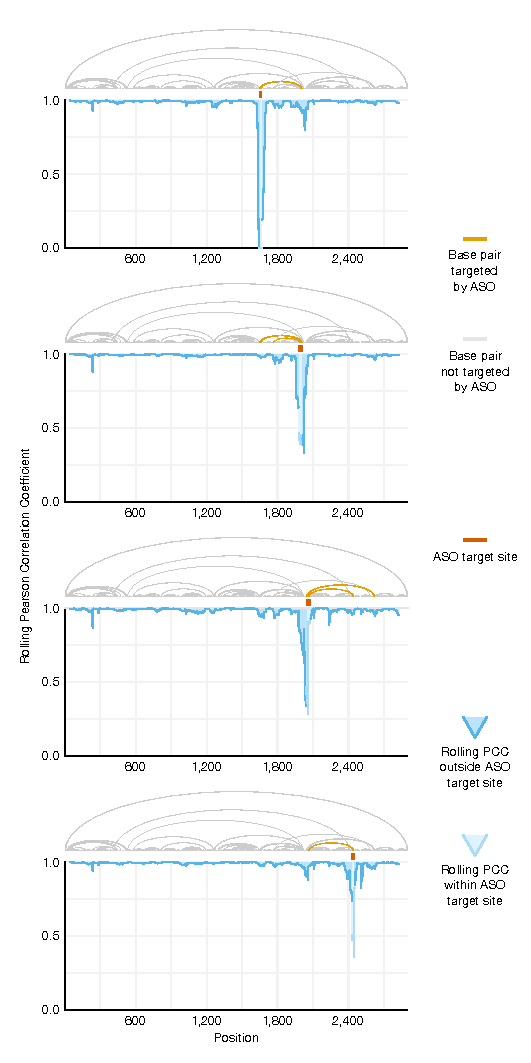
\includegraphics[width=0.5\textwidth]{../MainFigures/rrna/rrna.pdf}
	\caption{\textbf{Validation of SEARCH-MaP on 23S ribosomal RNA from \textit{E.~coli}.} Each graph shows the rolling (window = 45 nt) Pearson correlation coefficient (PCC) between the rRNA to which one ASO was added and a no-ASO control. The known secondary structure of the 23S rRNA~\cite{Cannone2002} is drawn above the graph; base pairs with one side within the ASO target site are highlighted.}
	\label{rrna}
\end{figure}

We folded the 23S rRNA with each ASO, performed DMS-MaPseq over the entire transcripts, and compared ensemble average mutational profiles with and without ASOs using SEISMIC-RNA (Figure~\ref{rrna}).
Every ASO caused a prominent dip in the rolling Pearson correlation coefficient (PCC) at its target site and the immediate vicinity, confirming that each ASO bound properly to the RNA.
The ASO targeting positions 1,647-1,668 also caused a smaller dip in PCC around positions 1,987-2,045 -- coinciding with the 3' side of a stem whose 5' side was targeted by the ASO -- showing that this stem could be detected with SEARCH-MaP.
Conversely, targeting the 3' side of this stem with an ASO binding positions 1,978-2,010 caused a small -- though still above-baseline -- dip in PCC around position 1,670 (near the stem's 5' side) and another around position 1,800 (the 5' side of another stem targeted by the ASO).
Shifting the ASO slightly downstream to target positions 2,042-2,076 maintained the dips in PCC around 1,670 and 1,800 while introducing new dips around positions 2,245, 2,435, and 2,630, which correspond to the 3' sides of three stems within or close to the ASO target site.
Binding an ASO to 2,429-2,452 -- the 3' side of one such stem -- caused the PCC to dip around position 2,055 at the 5' end of this stem.
These results show that SEARCH-MaP could detect multiple stems ranging from 200 to 600 nt in 23S rRNA from \textit{E.~coli}.

\subsection{SEARCH-MaP detects and quantifies long-range base pairing in SARS-CoV-2}

Aside from ribosomes, many of the best-characterized functional long-range RNA base pairs occur in the genomes of RNA viruses~\cite{Nicholson2014}.
Coronaviruses regulate translation of their first open reading frame (ORF1) using programmed ribosomal frameshifting~\cite{Plant2008}.
In the middle of ORF1, a switch called a frameshift stimulation element (FSE) makes a fraction of ribosomes slip backwards into the -1 reading frame.
Ribosomes that maintain reading frame terminate at a stop codon shortly after the FSE, while those that frameshift bypass that stop codon and reach the end of ORF1.
Why coronaviruses need a frameshifting mechanism remains an open question~\cite{Allan2023}, yet all have FSEs~\cite{Plant2008}.

Every coronaviral FSE contains a ``slippery site" (UUUAAAC) and a structure characterized as a pseudoknot in multiple species~\cite{Brierley1989,Herald1993,Plant2005b}.
Indeed, the isolated core of the FSE in SARS-CoV-2 was shown to fold into a pseudoknot with three stems~\cite{KZhang2021,Roman2021,Jones2022}.
However, we discovered that when FSE is in its natural place in the SARS-CoV-2 genome, pseudoknot stem 1 is disassembled while an alternative stem 1 folds~\cite{Lan2022}.
A 283 nt segment of the RNA genome -- containing both the FSE and alternative stem 1 -- failed to fully mimic the DMS reactivities of the full virus (PCC~=~0.75).
A 2,924 nt segment came closer (PCC~=~0.93), suggesting that -- only in the context of this longer sequence -- the FSE adopts yet another structure, presumably long-range base-pairing~\cite{Lan2022}.

We used SEARCH-MaP and SEISMIC-RNA to find the long-range base pairs formed by the FSE.
We hypothesized they would match a structure another group had discovered and named the ``FSE-arch"~\cite{Ziv2020}.
If so, the structure of the FSE would be perturbed by -- and only by -- ASOs targeting either side of the putative FSE-arch.
To investigate, we added (separately) thirteen groups of DNA ASOs to the 2,924 nt segment (Figure~\ref{tiles}a).
Each group contained four or five ASOs targeting a contiguous 213-244 nt section of the RNA; target sites of adjacent groups abutted without overlapping.
After adding each group of ASOs, we performed DMS-MaPseq~\cite{Zubradt2016} with two pairs of RT-PCR primers.
With the first pair of primers, flanking the ASO target site, we confirmed that the DMS reactivities were suppressed -- hence the ASO groups bound -- except for group 13, for which we obtained no data (Supplementary Figure~\ref{sars2-tile-target}).
With the second pair of primers, flanking the 5' side of the FSE-arch, we investigated how its structure was perturbed by each ASO group (Supplementary Figure~\ref{sars2-tile-fse}).

To quantify structural changes over the 5' FSE-arch, we calculated the rolling Pearson correlation coefficient (PCC) of the DMS reactivities between each sample and a no-ASO control (Figure~\ref{tiles}b).
The rolling PCC of a no-ASO replicate remained between 0.93 and 1.00 (mean~=~0.97), confirming the DMS reactivities were reproducible.
ASO group 9 -- targeting both 3' inner stems of the FSE-arch -- caused the rolling PCC to dip below 0.5 over both 5' inner stems, exactly as expected if the inner stems of the FSE-arch existed.
The only other ASO groups with substantial effects were 3, 4, and 5, which overlapped or abutted the FSE and presumably perturbed short-range base pairs; the outer stem of the FSE-arch (targeted by ASO group 10) did not apparently form.
These results suggest both inner stems of the FSE-arch exist and are the predominant long-range base pairs involving the immediate vicinity of the FSE.

\begin{figure}[H]
	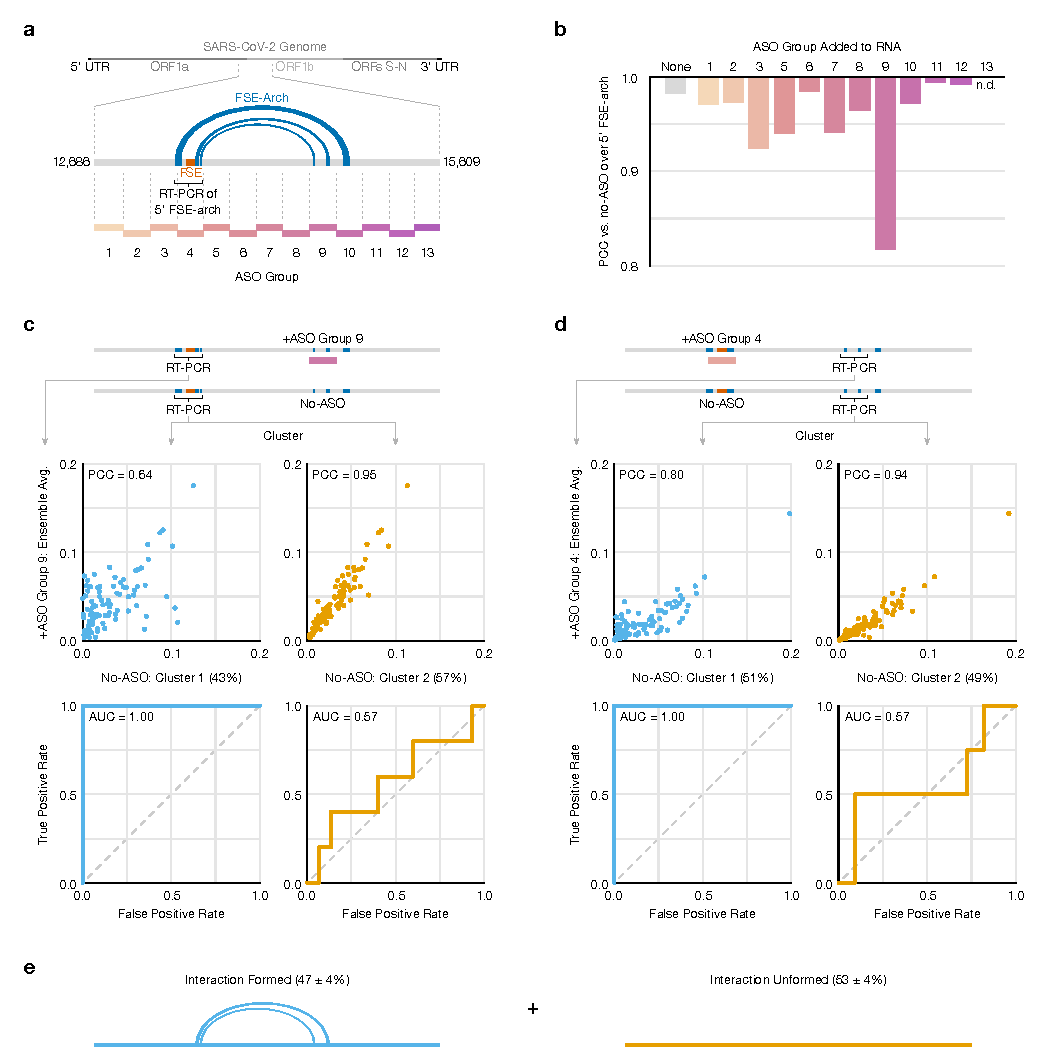
\includegraphics[width=\textwidth]{../MainFigures/sars2-tile/sars2-tile.pdf}
	\caption{\textbf{Search for a long-range base pairs involving the SARS-CoV-2 FSE.} \textbf{(a)}~The 2,924 nt segment of the SARS-CoV-2 genome containing the frameshift stimulation element (FSE) and putative FSE-arch~\cite{Ziv2020}. The target site for each group of antisense oligonucleotides (ASOs) is indicated by dotted lines; lengths are to scale. \textbf{(b)}~Rolling (window~=~45 nt) Pearson correlation coefficient (PCC) of DMS reactivities over the 5' FSE-arch between each +ASO sample and a no-ASO control. Each curve represents one ASO group, colored as in (a); groups 4 and 13 are not shown. Locations of the FSE and the outer and inner stems of the 5' FSE-arch are also indicated. \textbf{(c)}~(Top) Scatter plots of DMS reactivities over the 5' FSE-arch comparing each cluster of the no-ASO sample to the sample with ASO group 9; each point is one position in the 5' FSE-arch. (Bottom) Receiver operating characteristic (ROC) curves comparing each cluster of the no-ASO sample to the two inner stems of the FSE-arch, with area under the curve (AUC) indicated. \textbf{(d)}~Like (c) but over the 3' FSE-arch, and comparing to the sample with ASO group 4. One highly reactive outlier was ignored when calculating PCC (which is sensitive to outliers) but included in the ROC (which is robust). \textbf{(e)}~Model of the inner two stems in the ensemble of structures formed by the 2,924 nt segment.}
	\label{tiles}
\end{figure}

We next sought to determine the fraction of molecules in which the two inner stems of the FSE-arch form.
Using SEISMIC-RNA, we clustered reads from the 5' side of the FSE-arch for the no-ASO control and found two clusters with a 43/57\% split.
To determine if they corresponded to the two inner stems formed and unformed, we compared their DMS reactivities to those after adding ASO group 9, which blocks the two inner stems (Figure~\ref{tiles}c, top).
Cluster 2 had similar DMS reactivities (PCC~=~0.95), indicating it corresponds to the stems unformed.
Meanwhile, the DMS reactivities of cluster 1 differed (PCC~=~0.64), suggesting it corresponds to the stems formed.

To further support this result, we leveraged the preexisting model of the FSE-arch~\cite{Ziv2020}.
If cluster 1 did correspond to the two inner stems formed, its DMS reactivities would agree well with their structures (i.e. paired and unpaired bases should have low and high reactivities, respectively), while those of cluster 2 would agree less.
We quantified this agreement using receiver operating characteristic (ROC) curves (Figure~\ref{tiles}c, bottom).
The area under the curve (AUC) for cluster 1 was 1.00, indicating perfect agreement with the two inner stems of the FSE-arch; while that of cluster 2 was 0.57, close to no agreement (0.50).
This result further supports that clusters 1 and 2 correspond to the two inner stems formed and unformed, respectively.

If the RNA did exist as an ensemble of the two inner stems formed and unformed, the 3' side of the FSE-arch would also cluster into formed and unformed states.
To investigate, we performed RT-PCR with primers flanking the 3' side of the inner two stems -- both without ASOs and with ASO group 4 (targeting the 5' side of the FSE-arch).
We clustered the no-ASO control into two clusters (51/49\% split) and found -- similar to the previous result -- that the DMS reactivities after blocking the 5' FSE-arch with ASO group 4 resembled those of cluster 2 (PCC~=~0.94) but not cluster 1 (PCC~=~0.80), while the structure of the two inner stems agreed with cluster 1 (AUC~=~1.00) but not cluster 2 (AUC~=~0.57) (Figure~\ref{tiles}d).
We concluded that the RNA exists as an ensemble of structures in which the two inner stems of the FSE-arch form in 47\% ± 4\% of molecules (Figure~\ref{tiles}e).

\subsection{The long-range stems compete with the frameshift pseudoknot in SARS-CoV-2}

To determine if the FSE forms other long-range stems, in lieu of the original outer stem of the FSE-arch~\cite{Ziv2020}, we modeled a 1,799 nt segment centered on the FSE-arch.
Although computationally predicting long-range base pairs is notoriously unreliable~\cite{Doshi2004,Nicholson2015}, we speculated that we could improve accuracy by incorporating the DMS reactivities of cluster 1 on both sides of the FSE-arch (Supplementary Figure~\ref{sars2-clusters-fold}).
For the innermost stem -- which we call long stem 1 (LS1) -- nine of thirteen structures (69\%) predicted using the cluster 1 DMS reactivities contained LS1, compared to five of eleven (45\%) using the ensemble average and four of twenty (20\%) using no DMS reactivities.
For the second-most inner stem (LS2), eight structures (62\%) predicted using cluster 1 contained LS2, while none did using average or no DMS reactivities.
Thus, the DMS reactivities corresponding to the long-range cluster enabled predicting the long-range stems more consistently, allowing us to refine our model of the long-range stems.

Our refined model based on the long-range cluster (Figure~\ref{lnas}) included not only the two inner stems of the FSE-arch -- LS1 and LS2a/b -- but also two long stems (LS3a/b and LS4) that were not in the original FSE-arch model~\cite{Ziv2020}.
The structure also contained the alternative stem 1 (AS1) that we had previously discovered~\cite{Lan2022}.
To our surprise, LS2b, LS3, and LS4 of the refined model collectively overlapped all three stems of the pseudoknot (PS1, PS2, and PS3) that is thought to stimulate frameshifting~\cite{Kelly2020,KZhang2021,Jones2022}.
Thus, these long stems -- if they exist -- would be mutually exclusive with the pseudoknot.

To verify this refined model, we performed SEARCH-MaP on the 1,799 nt segment using 15-20 nt LNA/DNA mixmer ASOs for single-stem precision (Figure~\ref{lnas}b).
Each ASO targeted the 3' side of one stem, and we measured the change in DMS reactivities of the FSE.
ASOs targeting the 3' sides of LS1 and LS2a perturbed the DMS reactivities in exactly the expected locations on the 5' sides.
Binding an ASO to the 3' side of LS2b caused a larger perturbation with more off-target effects, likely because this stem overlaps with pseudoknot stem 2 (PS2).
Blocking LS3b also resulted in a main effect around the intended location, with one off-target effect upstream, suggesting that other base pairs between the pseudoknot and this upstream region may exist.
Therefore, stems LS1, LS2a/b, and LS3b do exist -- at least in a portion of the ensemble.

We then investigated whether the long-range stems compete with the pseudoknot.
If they did, blocking them with ASOs would increase the proportion of the pseudoknot in the ensemble.
To test this hypothesis, we first generated four possible models of the FSE structure by combining mutually compatible stems from the refined model (Figure~\ref{lnas}c).
Then, we clustered the 1,799 nt segment without ASOs up to 6 clusters -- the maximum number reproducible between replicates -- (Supplementary Figure~\ref{sars2-compare-clusters}a) and compared each cluster to each structure model using the area under the receiver operating characteristic curve (AUC-ROC) over the positions spanned by the pseudoknot, 305-371 (Figure~\ref{lnas}d, top).
We considered a cluster and model to be ``consistent" if the AUC-ROC was at least 0.90.
The locally nested model (AS1 plus PS2 and PS3) was consistent with three clusters totaling 52\% of the ensemble, while the extended model (AS1 plus all long-range stems) was consistent with one cluster (20\%).
No clusters were fully consistent with the pseudoknotted model, though the least-abundant cluster (7\%) came close with an AUC-ROC of 0.88.
The remaining cluster (21\%) was not consistent with any model, suggesting that the ensemble contains structures beyond those in Figure~\ref{lnas}c.

Adding an ASO targeting the 5' side of AS1 reduced the proportion of AS1-containing states (extended and locally nested) from 72\% to 16\% (Figure~\ref{lnas}d, left; Supplementary Figure~\ref{sars2-compare-clusters}b).
In their absence emerged clusters consistent with the pseudoknotted and truncated models, constituting 56\% and 20\% of the ensemble, respectively.
Meanwhile, adding an ASO that blocked the part of LS2b that overlaps PS2 eliminated the extended state (which includes LS2b) and produced one cluster (13\%) consistent with the pseudoknotted model (Figure~\ref{lnas}d, right; Supplementary Figure~\ref{sars2-compare-clusters}c).
Adding both ASOs simultaneously collapsed the ensemble into three clusters of which two (87\%) were highly consistent with the pseudoknotted model (Figure~\ref{lnas}d, bottom; Supplementary Figure~\ref{sars2-compare-clusters}d).
Since blocking the PS2-overlapping portion of LS2b increased the proportion of clusters consistent (or nearly so) with the pseudoknotted model -- both alone and combined with the anti-AS1 ASO -- we conclude that the long-range stems do outcompete the pseudoknot.

\begin{figure}[H]
	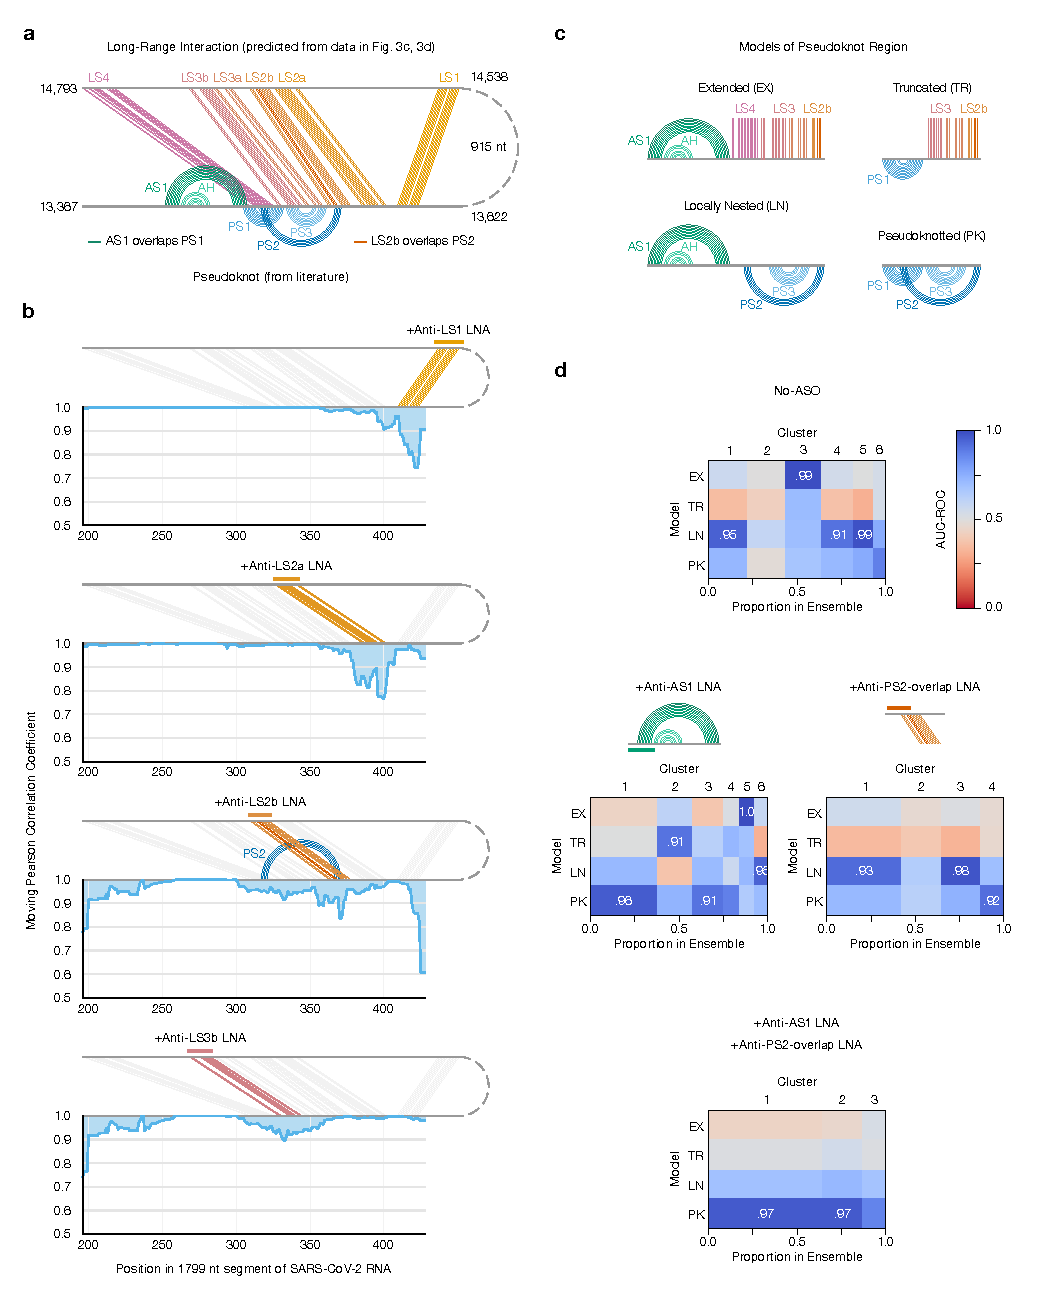
\includegraphics[width=\textwidth]{../MainFigures/lnas/lnas.pdf}
	\caption{\textbf{Refinement of the long-range structure model and competition with the frameshift pseudoknot.} \textbf{(a)}~Refined model of the long-range stems (minimum free energy prediction based on cluster 1 in Figure~\ref{tiles}c and d) including alternative stem 1 (AS1)~\cite{Lan2022}; the attenuator hairpin (AH)~\cite{Su2005}; and long stems LS1, LS2a/b, LS3a/b, and LS4. Locations of pseudoknot stems PS1, PS2, and PS3 are also shown; as are the base pairs they overlap in AS1 and LS2b. \textbf{(b)}~Rolling (window~=~21 nt) Pearson correlation coefficient of DMS reactivities between each +ASO sample and a no-ASO control; base pairs targeted by each ASO are colored. \textbf{(c)}~Models of possible structures for the FSE, by combining non-overlapping stems from (a). \textbf{(d)}~Heatmaps comparing models in (c) to clusters of DMS reactivities over positions 305-371 via the area under the receiver operating characteristic curve (AUC-ROC). AUC-ROCs at least 0.90 are annotated. Cluster widths indicate proportions in the ensemble.}
	\label{lnas}
\end{figure}

\subsection{Frameshift stimulating elements of multiple coronaviruses form long-range base pairs}

We hypothesized that other coronaviruses would also feature long-range base pairs involving the FSE.
To search for these structures, we performed SEARCH-MaP with FSE-targeted ASOs on 1,799 nt segments from eight coronaviral genomes.

As of December 2021, the NCBI Reference Sequence Database~\cite{OLeary2016} contained 62 complete genomes of coronaviruses.
To focus on those likely to have long-range base pairs involving the FSE, we predicted the likelihood that each base in a 2,000 nt section surrounding the FSE would pair with a base in the FSE (Supplementary Figure~\ref{contact_freqs}).
Based on these predicted structures, we selected ten coronaviruses -- at least one from each genus (Supplementary Figure~\ref{ten-covs}a) -- including SARS-CoV-2 as a positive control.
Within the genus \textit{Betacoronavirus}, we included all three SARS-related viruses -- SARS coronaviruses 1 (\verb|NC_004718.3|) and 2 (\verb|NC_045512.2|) and bat coronavirus BM48-31 (\verb|NC_014470.1|) -- because they clustered into their own structural outgroup.
The other three strains of \textit{Betacoronavirus} that we selected were MERS coronavirus (\verb|NC_019843.3|) with predicted base pairs at positions 510-530; and human coronavirus OC43 (\verb|NC_006213.1|) and murine hepatitis virus strain A59 (\verb|NC_048217.1|), both with a predicted upstream base pairs at positions 10-20.
We selected two strains of \textit{Alphacoronavirus}: transmissible gastroenteritis virus (\verb|NC_038861.1|) and bat coronavirus 1A (\verb|NC_010437.1|), predicted to have base pairs at positions 440-460 and 350-360, respectively.
For avian infectious bronchitis virus strain Beaudette (\verb|NC_001451.1|) -- a strain of \textit{Gammacoronavirus} -- the FSE was predicted to base-pair with positions 330-350; while common moorhen coronavirus HKU21 (\verb|NC_016996.1|) was the species of \textit{Deltacoronavirus} with the most promising long-range base pairs.

We reasoned that if an FSE does interact with a distant RNA element, removing that element by truncating the RNA would change the structure of the FSE, which we could detect with DMS-MaPseq~\cite{Zubradt2016}.
For each of the ten coronaviruses that passed the computational screen, we \textit{in vitro} transcribed and performed DMS-MaPseq on both a 239 nt segment comprising the FSE and minimal flanking sequences and a 1,799 nt segment encompassing the FSE and all sites with which it was predicted to interact.
All coronaviruses except for human coronavirus OC43 and MERS coronavirus showed differences in their DMS reactivity profiles between the 239 nt and 1,799 nt segments (Supplementary Figure~\ref{ten-covs}b), suggesting the FSE forms long-range base pairs.

To determine which RNA elements the FSE base-pairs with in each coronavirus, we performed SEARCH-MaP on the 1,799 nt RNA segment using DNA ASOs targeting the vicinity of the FSE (Figure~\ref{covs}).
The rolling Spearman correlation coefficient (SCC) between the +ASO and no-ASO mutational profiles dipped below 0.9 at the ASO target site in every coronavirus segment, confirming the ASOs bound and altered the structure.

To confirm we could detect long-range base pairs, we compared the rolling SCC for the SARS-CoV-2 segment to our refined model of the FSE structure (Figure~\ref{covs}, blue).
The SCC dipped below 0.9 at positions 1,483-1,560 and at 1,611-1,642, which coincide with stems LS2-LS3 (positions 1,476-1,550 within the 1,799 nt segment) and stem LS4 (positions 1,600-1,622).
These dips were the two largest downstream of the FSE; although others (corresponding to no known base pairs) existed, they were barely below 0.9 and could have resulted from base pairing between these regions and other (non-FSE) regions.
Near LS1 (positions 1,367-1,381), the SCC dipped only slightly to a minimum of 0.95, presumably because LS1 is the smallest (15 nt) and most isolated long-range stem.
Therefore, this method was sensitive enough to detect all but the smallest long-range stem, and specific enough that the two largest dips corresponded to validated long-range stems.

We found similar long-range stems in SARS-CoV-1 and another SARS-related virus, bat coronavirus BM48-31.
Both viruses showed dips in SCC at roughly the same positions as LS2-LS4 in SARS-CoV-2, indicating that they have homologous structures.
SARS-CoV-1 also had a wide dip below 0.9 at positions 1,284-1,394, corresponding to a homologous LS1.
Thus, three SARS-related viruses share these long-range stems involving the FSE, hinting that these structures are functional.

\begin{figure}[H]
	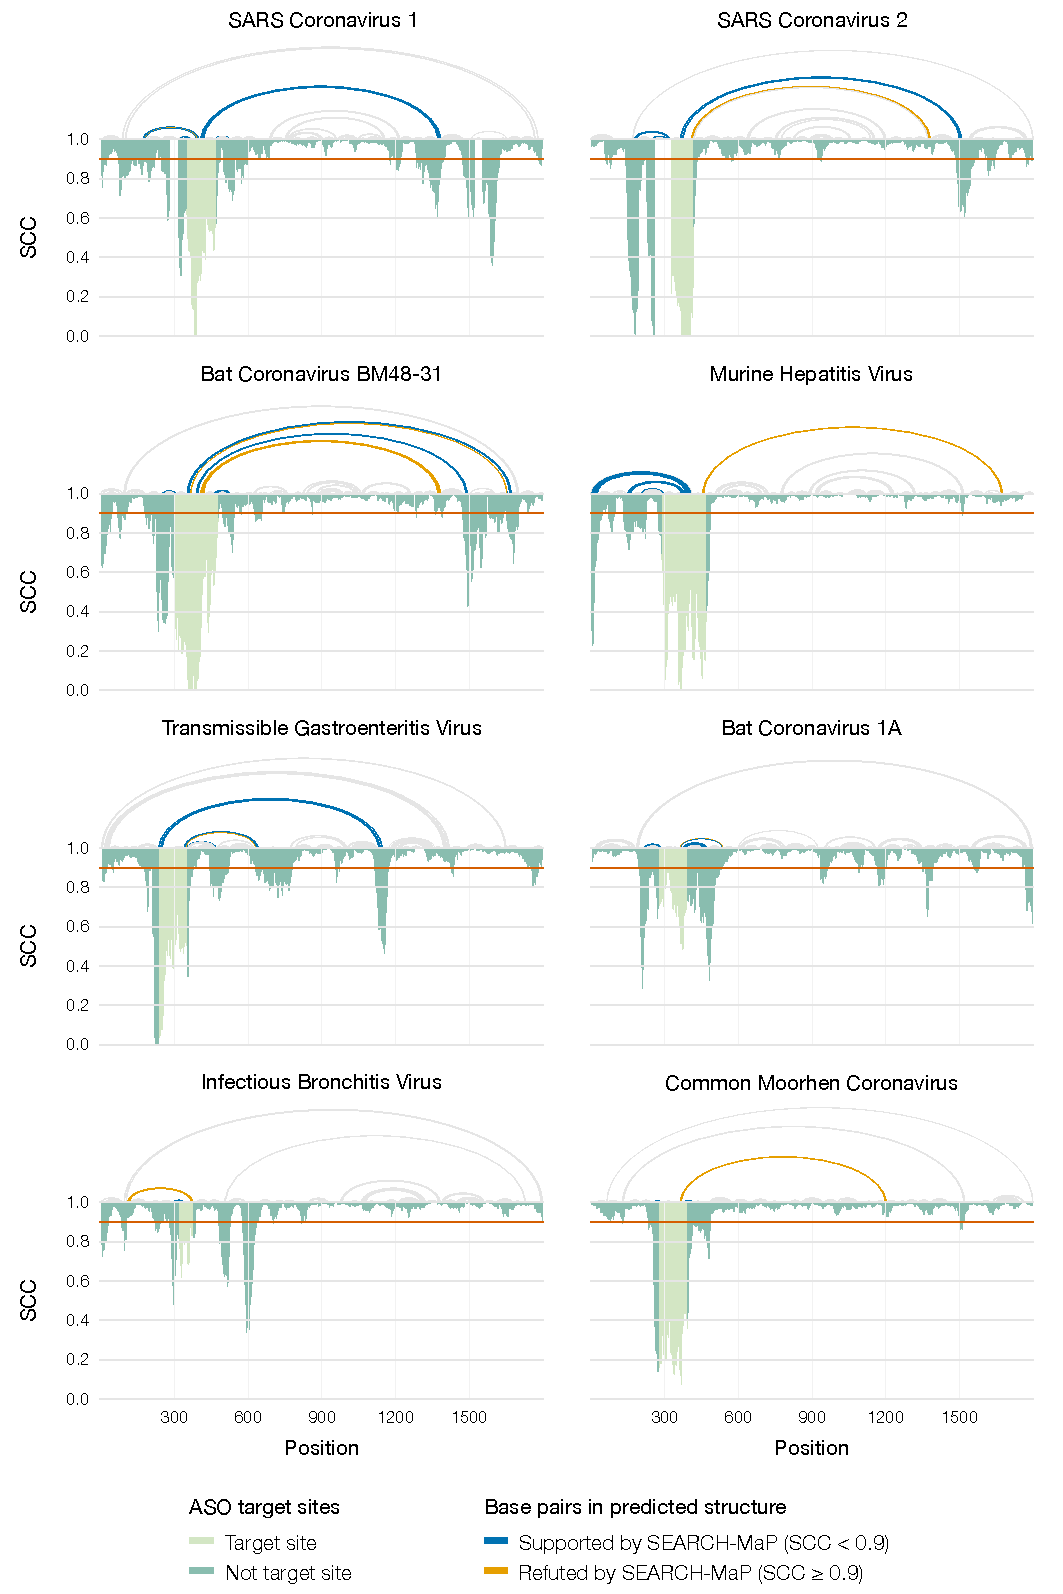
\includegraphics[width=\textwidth]{../MainFigures/covs/covs.pdf}
	\caption{\textbf{Evidence for long-range RNA--RNA base pairs involving the FSE in four additional coronaviruses.} Rolling (window~=~45 nt) Spearman correlation coefficient (SCC) of DMS reactivities between the +ASO and no-ASO samples for each 1,799 nt segment of a coronaviral genome. The target site of each ASO is highlighted on the SCC data and shown above each graph. Structures predicted with RNAstructure~\cite{Mathews2004a} using no-ASO ensemble average DMS reactivities as constraints~\cite{Cordero2012} are drawn above each graph; base pairs connecting the ASO target site to an off-target position with SCC less than 0.9 are colored. For SARS-CoV-2, the refined model (Figure~\ref{lnas}a) is also drawn, with LS1-LS4 labeled.}
	\label{covs}
\end{figure}

In every other species except common moorhen coronavirus, we found prominent dips in SCC at least 200 nt from the ASO target site.
To model potential base pairing between these dip positions and the FSE, we used the Fold program from RNAstructure~\cite{Mathews2004a} with the no-ASO ensemble average DMS reactivities as constraints~\cite{Cordero2012}.
We surmised that using the DMS reactivities corresponding to the long-range base pairs formed would generally yield more accurate predictions of the long-range structure than would using the ensemble average DMS reactivities (a mixture of all structures).
For instance, the prediction for SARS-CoV-2 based on the ensemble average included LS1 and LS2b but missed the other long-range stems.
Although clustered data were unavailable in this case, we were still able to find long-range base pairs consistent with the SEARCH-MaP data for both murine hepatitis virus and transmissible gastroenteritis virus (Figure~\ref{covs}, orange).
We conclude that long-range base pairing involving the FSE occurs more widely than in just SARS-CoV-2, including in the genus \textit{Alphacoronavirus}.

\subsection{Structure of the full TGEV genome in ST cells supports long-range base pairing involving the FSE}

Transmissible gastroenteritis virus (TGEV) is a strain of \textit{Alphacoronavirus 1}~\cite{Whittaker2018} that infects pigs and causes vomiting and diarrhea -- almost always fatally in baby piglets~\cite{Liu2021}.
Due to the impacts of TGEV on animal health and economics~\cite{Liu2021} and our evidence of a long-range stem, we sought to model the genomic secondary structures of live TGEV.
We began by treating TGEV-infected ST cells with DMS (two biological replicates) and performing DMS-MaPseq~\cite{Zubradt2016} (two technical replicates per biological replicate) on the extracted RNA (Figure~\ref{tgev}a).
The DMS reactivities over the full genome were consistent between biological replicates (PCC~=~0.97), albeit not with the 1,799 nt segment \textit{in vitro} (PCC~=~0.82), which showed that verifying the long-range stem in live TGEV would be necessary (Supplementary Figure~\ref{tgev_reps}).

To determine the structure ensembles, we performed RT-PCR on the extracted RNA using primers targeting both sides of the long-range stems.
The DMS reactivities from RT-PCR were consistent with those over the full genome (Supplementary Figure).
For each side of the long-range stem, we clustered the reads into two clusters (Figure~\ref{tgev}b).
These clusters had similar correlations with the +ASO sample and similar AUC-ROC scores (Supplementary Figure), making it more difficult to identify them for TGEV than for SARS-CoV-2 (Figure~\ref{tiles}).
Nevertheless, we realized that on each side, the bases that were predicted to interact had generally lower DMS reactivities in one cluster compared to the other cluster, and hypothesized that this cluster corresponded to the long-range stem formed (Figure~\ref{tgev}b).
On the 5' side, the less-reactive cluster constituted 52\% of the ensemble; on the 3' side, 60\%.
To investigate, we refined the structure of the 1,799 nt segment using the DMS reactivities from both of these clusters.
Consistent with our hypothesis, the minimum free energy (MFE) model included the long-range stem, which we hereafter call long stem 3 (LS3) (Figure~\ref{tgev}c); predicting the structure using both more-reactive clusters did not produce LS3 (Supplementary Figure).
The refined model also featured a prominent new stem connecting 20 nt upstream of the FSE with 400 nt downstream, which we call LS2.
We suspect that LS2 exists because it coincides with a broad region perturbed by adding an ASO to the FSE in the 1,799 nt segment of TGEV (Figure~\ref{tgev}c).
Another stem spanning just under 300 nt, which we call LS1, was also predicted in the same location as in the 1,799 nt segment.

\begin{figure}[H]
	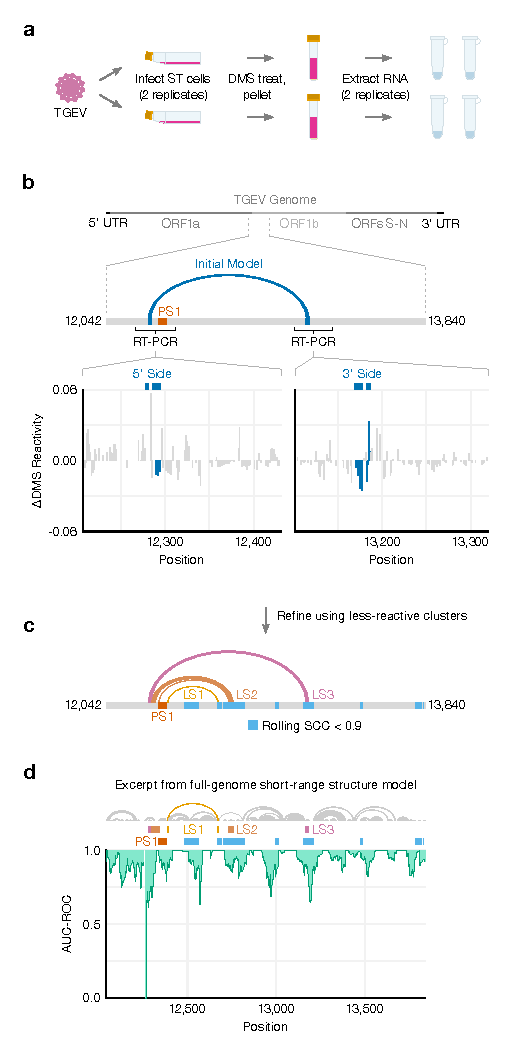
\includegraphics[width=0.5\textwidth]{../MainFigures/tgev/tgev.pdf}
	\caption{\textbf{Genomic secondary structure of live TGEV.} \textbf{(a)}~Schematic of the experiment in which two biological replicates of ST cells were infected with TGEV, DMS-treated, and pelleted. Cell pellets were divided into two technical replicates prior to extraction of DMS-modified RNA. \textbf{(b)}~Differences in DMS reactivities between the two clusters on each side of the long-range stem. Each bar represents one base. Bases are shaded dark blue if they pair in the initial model of the long-range stem (from Figure~\ref{covs}), shown above along with its location in the full genome. The locations of FSE pseudoknot stem 1 (PS1) and the regions amplified for clustering are also indicated. \textbf{(c)}~Refined model of the long-range stem in TGEV based on the DMS reactivities of the less-reactive cluster from both sides. Long stems 1 (LS1), 2 (LS2), and 3 (LS3) are labeled. For comparison with the regions of the 1,799 nt segment perturbed by the ASO (Figure~\ref{covs}), positions after the FSE where the Spearman correlation coefficient (SCC) dipped below 0.9 are shaded light blue. \textbf{(d)}~Rolling AUC-ROC (window = 45 nt) between the full-genome DMS reactivities and full-genome secondary structure modeled from the DMS reactivities (maximum 300 nt between paired bases). The structure model is drawn above the graph. Only positions 12,042-13,840 are shown here. For comparison, the locations of PS1, LS1, LS2, LS3, and dips in SCC after the FSE are also indicated.}
	\label{tgev}
\end{figure}

We used the ensemble average DMS reactivities to produce one ``ensemble average" model of the secondary structure of the full TGEV genome (Supplementary Figure).
We restricted base pairs to a maximum distance of 300 nt to make the computation tractable and avoid over-predicting spurious long-range base pairs.
To verify the model quality, we confirmed that the predicted structure of the first 520 nt included the highly conserved stem loops SL1, SL2, SL4, and SL5a/b/c in the 5' UTR~\cite{Yang2015a} (Supplementary Figure~\ref{tgev_5utr}a) and was consistent with the DMS reactivities (AUC-ROC = 0.94) (Supplementary Figure~\ref{tgev_5utr}b).

The AUC-ROC was lower in many locations throughout the rest of the genome (Supplementary Figure), indicating that a single secondary structure consistent with the ensemble average DMS reactivities could not be found.
We had noticed a similar phenomenon in SARS-CoV-2 -- in particular, at the FSE~\cite{Lan2022}.
Thus, we surmised that regions with low AUC-ROC scores likely form alternative structures or long-range base pairs -- or both -- that a single secondary structure model could not capture.
Checking if this relationship also held for TGEV, we found a large dip in AUC-ROC just upstream of the FSE, centered on the 5' ends of LS2 and LS3, as well as smaller dips at the 3' ends of both stems (Figure~\ref{tgev}d).
In fact, at or near every location that SEARCH-MaP had evidenced to interact with the FSE -- where the rolling SCC had dipped -- the AUC-ROC also dipped.
This finding supports the hypothesis that long-range base pairs and/or alternative structures are often the reason why predicted structures are not locally consistent with the DMS reactivities on which they were based.


\end{document}
